\documentclass{article}
\usepackage[T1]{fontenc}
\usepackage{lmodern}
\usepackage{graphicx}
\usepackage{amsmath,amssymb}
\usepackage[a4paper,margin=2cm]{geometry}
\usepackage[absolute,overlay]{textpos}
\setlength{\TPHorizModule}{1mm}
\setlength{\TPVertModule}{1mm}
\usepackage[indonesian]{babel}
\usepackage{hyperref}
\setlength{\emergencystretch}{2em}
% unit: Halaman 77

\begin{document}

% === Halaman 77 (llm) ===

\vspace{148.50mm}

\begin{verbatim}
# Ubah 8-bit pesan ke dalam setiap karakter
pesan = ""
for i in range(len(bit_pesan)):
    if pesan[-5:] == "#####": # ketemu delimiter
        break
    else:
        pesan = pesan + chr(int(bit_pesan[i], 2))

if "#####" in pesan:
    print("Pesan yang diekstraksi:", pesan[:-5])
else:
    print("Tidak ada pesan tersembunyi di dalam citra")
\end{verbatim}

% deskripsi: Screenshot cuplikan kode Python untuk mengekstraksi pesan dari rangkaian bit, dengan pengecekan delimiter '#####'.
% bbox normalisasi: [0.0500, 0.0500, 0.9400, 0.5500]
\begin{textblock*}{186.90mm}(10.50mm,14.85mm)
\noindent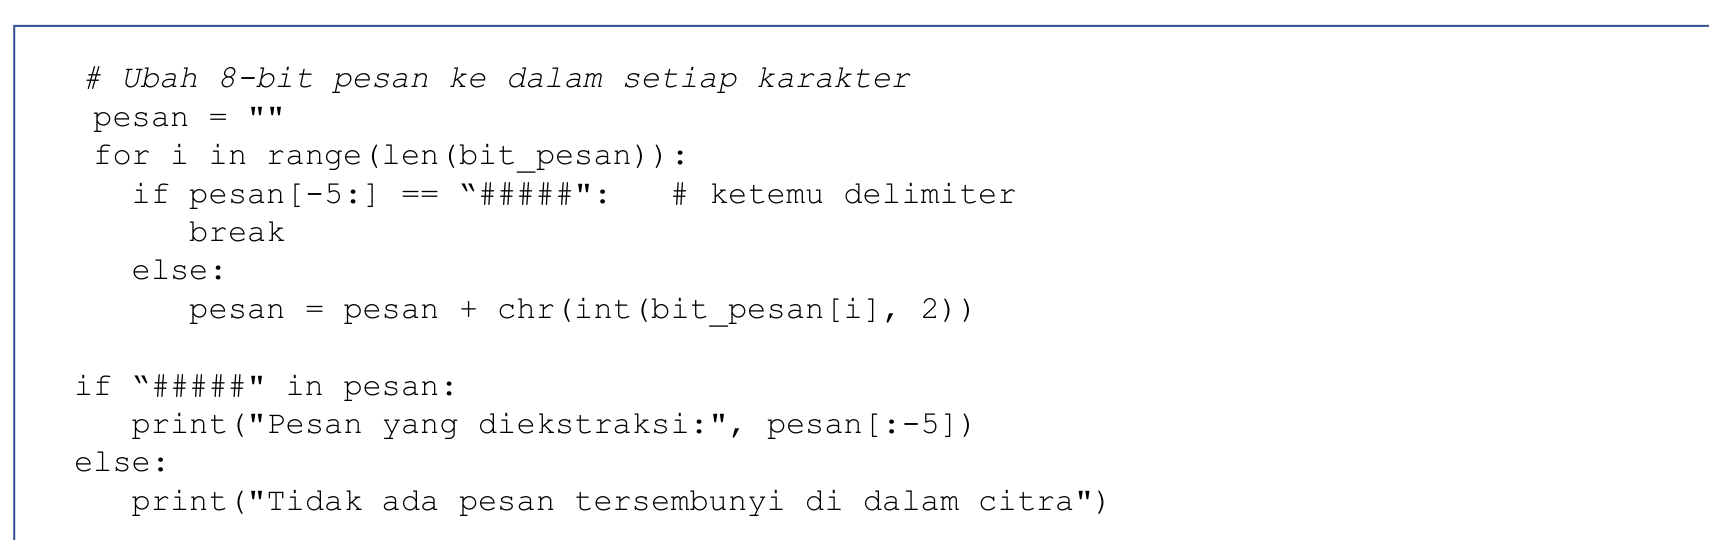
\includegraphics[width=186.90mm,height=148.50mm]{../../images/llm/page_077_img_01.png}%
\end{textblock*}

\end{document}
